\section{Experiments}
In this section, we evaluate our method on the most popular scene graph generation dataset, Visual Genome (VG). To demonstrate the effectiveness of our method, we compare it with several recent methods, including MOTIFS, VCTree, and BGNN. We also perform comprehensive ablation studies on different components and provide a discussion on different cost-sensitive methods for imbalance learning.
% We apply our method to several models including MOTIFS, VCTree, and DTrans for all SGG tasks.

\begin{table*}[!ht]
	\centering
% 	\scriptsize
    \small
     \setlength{\tabcolsep}{1mm}
	\begin{tabular}{c|ccc|ccc|ccc}
\hline
                                        & \multicolumn{3}{c|}{Predcls} & \multicolumn{3}{c|}{SGcls} & \multicolumn{3}{c}{SGdet} \\
Models                                  & mR@20   & mR@50   & mR@100   & mR@20   & mR@50  & mR@100  & mR@20   & mR@50  & mR@100  \\ \hline
KERN\ddag\cite{chen2019knowledge}       & -       & 17.7    & 19.2     & -       & 9.4    & 10.0    & -       & 6.4    & 7.3     \\
PCPL\ddag\cite{yan2020pcpl}             & -       & 35.2    & 37.8     & -       & 18.6   & 19.6    & -       & 9.5    & 11.7    \\
GPS-Net\ddag\cite{lin2020gps}           & 17.4    & 21.3    & 22.8     & 10.0    & 11.8   & 12.6    & 6.9     & 8.7    & 9.8     \\
BGNN\cite{li2021bipartite}              & -       & 30.4    & 32.9     & -       & 14.3   & 16.5    & -       & 10.7   & 12.6    \\ \hline
MOTIFS\dag\cite{Zellers_2018_CVPR}      & 13.6    & 17.2    & 18.6     & 7.8     & 9.7    & 10.3    & 5.6     & 7.7    & 9.2     \\
MOTIFS+TDE\cite{Tang2020_unbiased}      & 18.5    & 24.9    & 28.3     & 11.1    & 13.9   & 15.2    & 6.6     & 8.5    & 9.9     \\
MOTIFS+DLFE\cite{chiou2021recovering}   & 22.1    & 26.9    & 28.8     & 12.8    & 15.2   & 15.9    & 8.6     & 11.7   & 13.8    \\
MOTIFS + \textbf{RTPB(CB)}              & 28.8    & 35.3    & 37.7     & 16.3    & 19.4   & 20.6    & 9.7     & 13.1   & 15.5    \\ \hline
VCTree\dag\cite{VCTree_tang}            & 13.4    & 16.8    & 18.1     & 8.5     & 10.8   & 11.5    & 5.4     & 7.4    & 8.6     \\
VCTree+TDE\cite{Tang2020_unbiased}      & 17.2    & 23.3    & 26.6     & 8.9     & 11.8   & 13.4    & 6.3     & 8.6    & 10.3    \\
VCTree + DLFE\cite{chiou2021recovering} & 20.8    & 25.3    & 27.1     & 15.8    & 18.9   & 20.0    & 8.6     & 11.8   & 13.8    \\
VCTree+\textbf{RTPB(CB)  }              & 27.3    & 33.4    & 35.6     & \textbf{20.6}    & \textbf{24.5}   & \textbf{25.8}    & 9.6     & 12.8   & 15.1    \\ \hline
DTrans                                  & 15.1    & 19.3    & 21.0     & 9.9     & 12.1   & 13.0    & 6.6     & 9.0    & 10.8    \\
DTrans+\textbf{RTPB(CB) }               & \textbf{30.3}    & \textbf{36.2}    & \textbf{38.1 }    & 19.1    & 21.8   & 22.8    & \textbf{12.7 }   & \textbf{16.5}   & \textbf{19.0}    \\
DTrans+\textbf{RTPB(VB)}                & 25.5    & 31.1    & 33.3     & 17.3    & 20.1   & 21.3    & 11.9    & 15.7   & 18.4    \\
DTrans+\textbf{RTPB(PB)}                & 17.4    & 21.6    & 23.1     & 11.9    & 14.0   & 14.7    & 7.7     & 10.1   & 11.9    \\
DTrans+\textbf{RTPB(EB)}                & 22.7    & 26.7    & 28.4     & 15.2    & 17.4   & 18.2    & 11.0    & 14.1   & 16.1    \\ \hline
\end{tabular}
	%	\small
	\caption{ The performance on VG~\cite{krishna2016visual} under graph constraints setting. \dag~indicates the results reproduced using the code of \cite{Tang2020_unbiased}. \ddag~models are with VGG16 backbone \cite{simonyan2014very}, while others are with ResNeXt-101-FPN backbone \cite{Lin_2017_ICCV}. (CB), (VB), (PB), and (EB) indicate the count resistance bias, the valid resistance bias, the pair resistance bias, and the estimated resistance bias, respectively. 
% 	Besides, we put results of other metric and the visualization of the results in the Supp..
	}
	\label{tab:sgg-mr}
\end{table*}

\subsection{Dataset and Evaluation Metrics}

\subsubsection{Dataset} 
% We perform extensive experiments on Visual Genome (VG)~\cite{krishna2016visual} dataset. This dataset contains 108k images from 75k object categories and 37k predicate categories. Considering that many relationship categories in VG only have less than 10 samples, 
% similar to~\cite{Xu2017,Zellers_2018_CVPR,Tang2020_unbiased}, we use the widely adapted subset, VG150, which consists of the most frequent 150 object categories and 50 predicate categories. Specifically, we follow the original training/testing split, i.e., 70\% data samples for training and the rest 30\% for testing.
We perform extensive experiments on Visual Genome (VG)~\cite{krishna2016visual} dataset. Similar to previous work~\cite{Xu2017,Zellers_2018_CVPR,Tang2020_unbiased}, we use the widely adapted subset, VG150, which consists of the most frequent 150 object categories and 50 predicate categories. The original split only has training set (70\%) and test set (30\%). We follow \cite{Tang2020_unbiased} to sample a 5k validation set for parameter tuning.

%With different additional information, the SGG can be further divided into three sub-task: 1)Predicate Classification(PredCls), the input will include bounding boxes $(B)$ in the image and their labels $(O)$ in this task; 2)Scene graph classification(SGCls), it only gives the bounding boxes $(B)$; 3)Scene Graph Detection(SGDet), this task will provide no additional information.
\subsubsection{Evaluation Metrics}
For a fair comparison, we follow previous work~\cite{Zellers_2018_CVPR,Tang2020_unbiased,li2021bipartite} and evaluate the proposed method on three sub-tasks of scene graph generation as follows.
% According to the different additional information.
\begin{enumerate}
	\item Predicate Classification (\textbf{PredCls}). On this task, the input includes not only the image, but the bounding boxes in the image and their labels;
	\item Scene Graph Classification (\textbf{SGCls}). It only gives the bounding boxes;
	\item Scene Graph Detection (\textbf{SGDet}). On this task, no additional information other than the raw image will be given.
\end{enumerate}
For each sub-task, previous works use Recall@k (or R@k) to report the performance of scene graph generation~\cite{Lu16,Xu2017}, which indicates the recall rate of ground-truth relationship triplets (subject-predicate-object) among the top k predictions of each test image.
% In earlier work, Recall@k (R@k) was used to evaluate the SGG model, which measures the fraction of ground-truth relationship triplets (subject-predicate-object) that appear among in the k highest confidence predictions in an image. 
Considering that the above-mentioned metric (R@k) caters to the bias caused by the long-tailed distribution of object relationships, the model can only achieve a high recall rate by predicting the frequent relationships. Therefore, it can not demonstrate the effectiveness of different models on less frequent relationships. To this end, the mean recall rate of each relationships, (mR@k), has been widely used in recent works ~\cite{Zellers_2018_CVPR,VCTree_tang,Tang2020_unbiased,li2021bipartite}. Therefore, we report the performance using the mean Recall, and the results of Recall are available in the appendix.
%According to whether it is allowed to, both recall and mean recall can be divided into the one without graph constraint (ng-R@k, ng-mR@k) and the normal one with graph constraint (R@k, mR@k).

\subsection{Implementation Details}
We implement the proposed method using PyTorch~\cite{NEURIPS2019_9015}. For a fair comparison, we use the object detection model similar to \cite{Tang2020_unbiased}, i.e., a pretrained Faster RCNN with ResNeXt-101-FPN as the backbone network. The object detector is fine-tuned on the VG dataset. Then, we froze the object detector and train the rest parts of the SGG model.
% To fairly compare with other works, similar to previous work , we take ResNeXt-101-FPN as the backbone and use a pre-trained Fast RCNN as the detector, 
% which is kept frozen in the training phase of other parts of the SGG model. 
 For the DTrans, the number of object encoder layers is $n_o = 4$ and the number of relationship encoder layers is $n_r = 2$. For the proposed resistance bias, we use $a = 1$ and $\epsilon =0.001$ if not otherwise stated. For the background relationship, the bias is a constant value $log\frac{1}{\|\mathcal{C}_r\|} = log\frac{1}{50}$, where the $\mathcal{C}_r$ is the set of relationship labels. We perform our experiments using a single NVIDIA V100 GPU. We train the DTrans model for 18000 iterations with batch size 16. Specifically, it takes around 24 hours for the SGDet task, and less than 12 hours for the PredCls/SGCls task. For the SGDet task, we use all pairs of objects for training instead of those pair of objects with overlap. For other experimental settings, we always keep the same with the previous work~\cite{Tang2020_unbiased}.
%ResNeXt-101-FPN

\subsection{Comparison with Recent Methods}
To demonstrate the effectiveness of the proposed method, we apply RTPB on several representative methods for scene graph generation, including MOTIFS, VCTree, and our DTrans baseline model. 
% As shown in Table~\ref{tab:sgg-mr}, we find that RTPB can achieve consistent improvements on less frequent relationships when applying it on existing methods in terms of the mean recall rate. Since we aims to build a balanced model for scene graph generation, here we also report the performance using the mean recall rate. Specifically, RTPB may also lead to a slight performance degradation on the frequent relationships without overfitting on the head categories.
% As shown in Figure~\ref{fig:compR}, we find that the recall rate on most relationships have been significantly improved (DTrans w/o or w/ RTPB) on the SGDet task. Therefore, we see a clear improvement when using the mean recall rate as the evaluation metric.
As shown in Table~\ref{tab:sgg-mr}, we find that RTPB can achieve consistent improvements in the mean recall metric for all of MOTIFS, VCTree, and our DTrans. Models equipped with our RTPB achieve new state-of-the-art and out-preform previous methods by a clear margin. 
Take SGDet as an example, as shown in Figure~\ref{fig:compR}, the recall rate on most relationships has been significantly improved (DTrans w/o or w/ RTPB). Specifically, RTPB may also lead to slight performance degradation on the frequent relationships without over-fitting on the head categories. Therefore, we see a clear improvement when using the mean recall rate as the evaluation metric, which demonstrates RTPB can build a better-balanced model for unbiased SGG.

Among four instance of resistance bias, CB performs the best on mR because it simply calculates the relationship distribution based on the whole dataset. VB/PB/EB are proposed based on more critical conditions. Although we believe that adding more critical conditions would lead to more practical prior bias, currently, limited data are not sufficient to obtain proper empirical bias under the given conditions.
% How to obtain more useful prior bias is one of our future works. 



\begin{figure}[!ht]
	\centering
	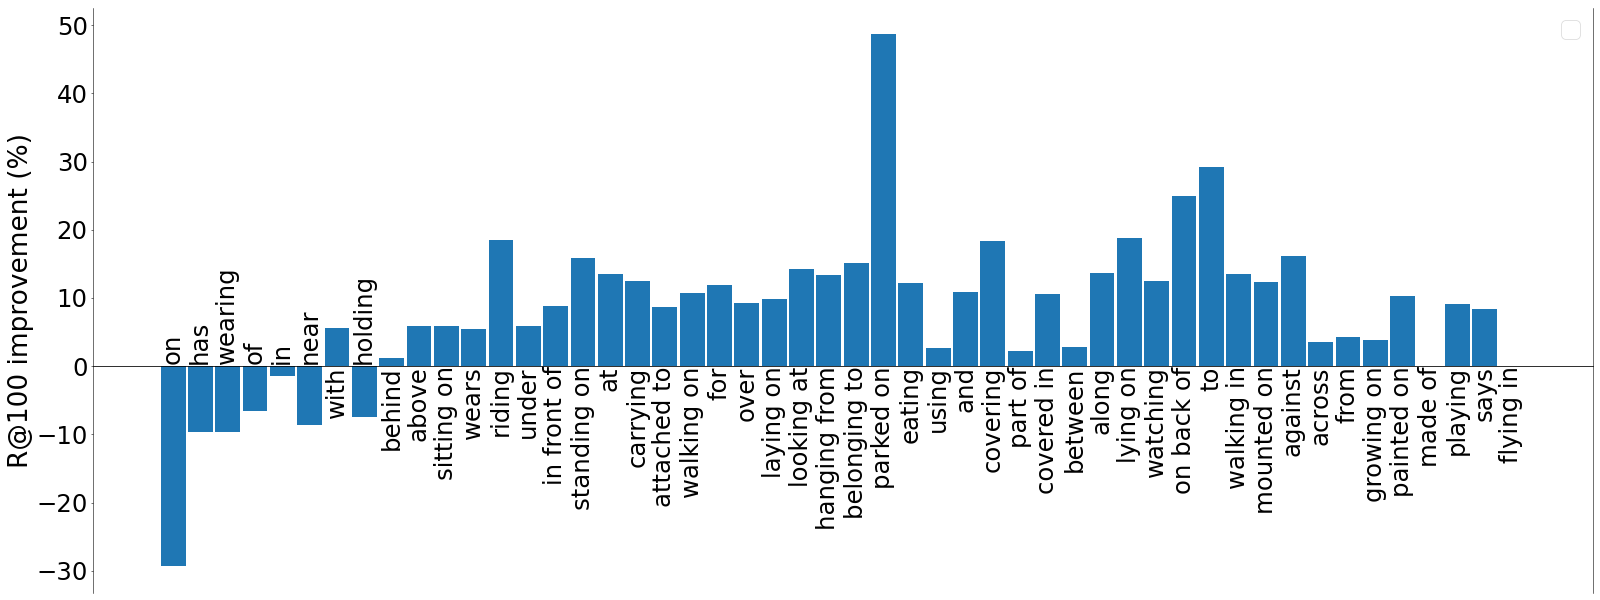
\includegraphics[width=\linewidth]{figure/compRecall} % Reduce the figure size so that it is slightly narrower than the column.
	\caption{The improvements of Recall@100 on the SGDet task using RTPB(CB). The number of relationships decreases from left to right. It shows that RTPB achieves higher recall rate on most relationships with a sacrifice on only a small number of frequent relationships.}
	\label{fig:compR}
\end{figure}